\section{Auswertung}
\label{sec:Auswertung}
Die in \autoref{sec:Auswertung} gezeigten Grafiken und Rechnungen sind mithilfe der Python-Bibliotheken Matplotlib \cite{matplotlib}, Scipy \cite{scipy} und Numpy \cite{numpy}
erstellt worden.%Vielleicht noch auskommentieren
%Fehlerrechnung noch hinzufügen

\subsection{Reflexionsgesetz}
\label{sec:Reflexionsgesetz}

\begin{table}
  \centering
  \caption{Messwerte für den Einfallswinkel $\alpha_1$ und den Ausfallswinkel $\alpha_2$ bei der Reflexion an einer ebenen Oberfläche.}
  \begin{tabular}{c c}
    \toprule
    $\alpha_1\,/\symup{°}$ & $\alpha_2\,/\symup{°}$ \\
    \midrule
    30 & 30.5\\
    35 & 35.5\\
    40 & 40.5\\
    45 & 45.5\\
    50 & 50.5\\
    60 & 60.5\\
    70 & 70.5\\
    \bottomrule
  \end{tabular}
  \label{tab:Reflexion}
\end{table}

Die Messwerte für den Einfallswinkel $\alpha_1$ und den Ausfallswinkel $\alpha_2$ sind in \autoref{tab:Reflexion} aufgelistet.
Die Winkel können mit einer Genauigkeit von $\pm\, 1\symup{°}$ abgelesen werden.
Dieser Fehler entspricht einer Skaleneinheit der Winkelskala. 
Die Genauigkeit ist für alle weiteren Versuchsteile gleich.

\subsection{Brechungsgesetz}
\label{sec:Brechungsgesetz}

\begin{table}
  \centering
  \caption{Messwerte für den Einfallswinkel $\alpha$ und den Brechungswinkel $\beta$ bei der Brechung einem optisch dichteren Medium.}
  \begin{tabular}{c c}
    \toprule
    $\alpha\,/\symup{°}$ & $\beta\,/\symup{°}$ \\
    \midrule
    10 & 7\\
    20 & 13.5\\
    30 & 20\\
    40 & 25.5\\
    50 & 31.5\\
    60 & 36\\
    70 & 39\\
    \bottomrule
  \end{tabular}
  \label{tab:Brechung}
\end{table}

Die Messwerte für den Einfallswinkel $\alpha$ und den Brechungswinkel $\beta$ sind in \autoref{tab:Brechung} aufgelistet.
Mit \autoref{eq:Brechungsgesetz} wird der Brechungsindex $n$ von Plexiglas bestimmt. 
Da das optisch dünnere Medium Luft ist, kann $n_1 = 1$ angenommen werden.

\begin{table}
  \centering
  \caption{Brechungsindex $n$ von Plexiglas mit Fehler.}
  \begin{tabular}{c}
    \toprule
    $n$ \\
    \midrule
    (1.42 \pm 0.25)\\
    (1.47 \pm 0.13)\\
    (1.46 \pm 0.08)\\
    (1.49 \pm 0.06)\\
    (1.47 \pm 0.05)\\
    (1.47 \pm 0.04)\\
    (1.49 \pm 0.03)\\
    \bottomrule    
  \end{tabular}
\end{table}
Gemittelt ergibt sich der Brechungsindex  $n_{\text{plexi}} = (1.47 \pm 0.02)$. 
Die Abweichung zum Literaturwert $n_{\text{plexi,lit}} = 1.49$ aus \autoref{tab:Brechungsindex} wird mit
\begin{equation*}
  \Delta = |\frac{exp - theo}{theo}|\cdot 100\%
\end{equation*}
berechnet und beträgt $1.5\%.$
Die Lichtgeschwindigkeit $c_{\text{M}}$ in einem Medium wird mit \autoref{eq:c_medium} berechnet.\\
In Plexiglas beträgt die Lichtgeschwindigkeit $c_{\text{plexi}} = \SI{2.043(0.033)e08}{\frac{m}{s}}$\\


\subsection{Planparallele Platten}
\label{sec:Planparallele Platten}

\begin{figure}
  \centering
  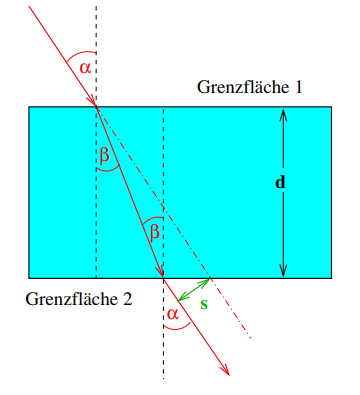
\includegraphics[width=0.5\textwidth]{img/strahlenversatz.png}
  \caption{Strahlenversatz bei der Brechung an einer planparallelen Platte.}
  \label{fig:Strahlenversatz}
\end{figure}

Die geometrische Herleitung des Strahlenversatzes $s$ ist in \autoref{fig:Strahlenversatz} dargestellt.
Der Strahlenversatz befindet sich in einem rechtwinkligen Dreieck mit der Hypotenuse $h$ und ist selbst die Gegenkathete des Winkels $\alpha - \beta$.
Da $h$ nicht bekannt ist wird es über den Satz des Pythagoras berechnet mit $d$ und $b$ als Katheten.
\begin{equation*}
  h = \sqrt{d^2 + b^2}
\end{equation*}
Die Kathete $b$ kann durch $b = d \cdot \tan(\beta)$ ausgedrückt werden.
Damit ergibt sich 
\begin{equation*}
  h = d \cdot \sqrt{1 + \tan^2(\beta)} = d \cdot \frac{1}{\cos(\beta)}.
\end{equation*}
Der Strahlenversatz $s$ ist dann
\begin{equation}\label{eq:Strahlenversatz}
  s = h \cdot \sin(\alpha - \beta) = d \cdot \frac{\sin(\alpha - \beta)}{\cos(\beta)}.
\end{equation}
\\
\\
Mithilfe der \autoref{eq:Strahlenversatz} wird der Strahlenversatz $s_1$ für die planparallele Platte mit den Werten aus \autoref{tab:Brechung} berechnet.
Wird $\beta$ über das Brechungsgesetz \eqref{eq:Brechungsgesetz} berechnet, so ergibt sich
\begin{equation*}
  \beta = \arcsin\left(\frac{\sin(\alpha)}{n}\right).
\end{equation*}
Mit dem in \autoref{sec:Brechungsgesetz} bestimmten Brechungsindex $n_{\text{plexi}}$ wird mit den $\alpha$-Werten aus \autoref{tab:Brechung} $\beta$ berechnet.
Daraus folgt der Strahlenversatz $s_2$.
\begin{table}
  \centering
  \caption{Strahlenversatz $s$ für die planparallele Platte mit \autoref{eq:Strahlenversatz} berechnet.}
  \begin{tabular}{c c c}
    \toprule
    {$s_1\,/\symup{mm}$} & {$\beta_{\text{calc}}\, / \symup{°}$} & {$s_2 \,/\symup{mm}$}\\
    \midrule
    3.1\pm 1.4 & 6.8\pm 0.7  & 3.3\pm 0.4 \\
    6.8\pm 1.5 & 13.5\pm 0.7 & 6.8\pm 0.4 \\
    10.8\pm 1.5 & 19.9\pm 0.7 & 10.9\pm 0.6 \\
    16.2\pm 1.5 & 26.0\pm 0.7 & 15.8\pm 0.7 \\
    21.8\pm 1.5 & 31.5\pm 0.8 & 21.8\pm 0.8 \\
    29.4\pm 1.4 & 36.2\pm 0.8 & 29.3\pm 1.0 \\
    38.8\pm 1.3 & 39.8\pm 0.8 & 38.3\pm 1.1 \\
    \bottomrule    
  \end{tabular}
\end{table}
Es zeigt sich, dass bei beiden Methoden das gleiche Ergebnis erzielt wird. 
Der Fehler der ersten Methode ist größer, als bei der Methode mit dem Brechungsgesetz.

\subsection{Prisma}
\label{sec:Prisma}

\begin{table}
  \centering
  \caption{Gemessene Einfallswinkel $\alpha$,\\ Brechungswinkel $\beta_{\text{grün}}$ und $\beta_{\text{rot}}$ am Prisma.}
  \begin{tabular}{c c c}
    \toprule
    {$\alpha\,/\symup{°}$} & {$\beta_{\text{grün}}\,/\symup{°}$} & {$\beta_{\text{rot}}\,/\symup{°}$}\\
    \midrule
    30 & 72.5 & 71.5\\
    35 & 62.5 & 62.0\\
    40 & 56.5 & 56.0\\
    50 & 45.5 & 45.0\\
    60 & 37.0 & 37.0\\
    70 & 31.0 & 31.0\\ 
    \bottomrule   
  \end{tabular}
\end{table}

Trifft ein Lichtstrahl auf ein Prisma, so wird er abhähgig von der Wellenlänge gebrochen.
Dieses Phänomen heißt Dispersion. 
Die Ablenkung des Strahles $\delta$, welche dieser beim Durchqueren des Prismas erfährt, wird berechnet mit
\begin{equation}
  \delta = (\alpha_1 + \alpha_2) - (\beta_1 + \beta_2).
\end{equation}
Es gilt die Winkelbeziehung $\beta_1 + \beta_2 = \gamma$. 
Weiter wird $\beta_1$ mithilfe des Brechungsgesetzes \eqref{eq:Brechungsgesetz} berechnet.
Der Brechungsindex wird $n = 1.55$ gewählt, als Wert für Kronglas aus \autoref{sec:Vorbereitungsaufgaben}.
Die Berechneten $\beta_1, \beta_2$ und $\delta$ sind in \autoref{tab:delta_gruen} und \autoref{tab:delta_rot} aufgelistet. 

\begin{table}
  \centering
  \caption{Ablenkung $\delta$, Einfallswinkel $\alpha_1$, Brechungswinkel $\beta_1$ und $\beta_2$ des grünen Laserstrahls beim Durchqueren des Prismas.}
  \begin{tabular}{c c c c c}
    \toprule
    {$\alpha_1\,/\symup{°}$} & {$\alpha_2\,/\symup{°}$} & {$\beta_1\,/\symup{°}$} & {$\beta_2\,/\symup{°}$} & {$\delta\,/\symup{°}$}\\
    \midrule
    (30.0\pm 1.0) & (72.5\pm 1.0) & (18.8\pm 0.6) & (41.2\pm 0.6) & (42.5\pm 1.4) \\
    (35.0\pm 1.0) & (62.5\pm 1.0) & (21.7\pm 0.6) & (38.3\pm 0.6) & (37.5\pm 1.4) \\
    (40.0\pm 1.0) & (56.5\pm 1.0) & (24.5\pm 0.5) & (35.5\pm 0.5) & (36.5\pm 1.4) \\
    (50.0\pm 1.0) & (45.5\pm 1.0) & (29.6\pm 0.5) & (30.4\pm 0.5) & (35.5\pm 1.4) \\
    (60.0\pm 1.0) & (37.0\pm 1.0) & (34.0\pm 0.4) & (26.0\pm 0.4) & (37.0\pm 1.4) \\
    \bottomrule
  \end{tabular}
  \label{tab:delta_gruen}
\end{table}

\begin{table}
  \centering
  \caption{Ablenkung $\delta$, Einfallswinkel $\alpha_1$, Brechungswinkel $\beta_1$ und $\beta_2$ des roten Laserstrahls beim Durchqueren des Prismas.}
  \begin{tabular}{c c c c c}
    \toprule
    {$\alpha_1\,/\symup{°}$} & {$\alpha_2\,/\symup{°}$} & {$\beta_1\,/\symup{°}$} & {$\beta_2\,/\symup{°}$} & {$\delta\,/\symup{°}$}\\
    \midrule
      (30.0\pm 1.0) & (71.5\pm 1.0) & (18.8\pm 0.6) & (41.2\pm 0.6) & (41.5\pm 1.4) \\
      (35.0\pm 1.0) & (62.0\pm 1.0) & (21.7\pm 0.6) & (38.3\pm 0.6) & (37.0\pm 1.4) \\
      (40.0\pm 1.0) & (56.0\pm 1.0) & (24.5\pm 0.5) & (35.5\pm 0.5) & (36.0\pm 1.4) \\
      (50.0\pm 1.0) & (45.0\pm 1.0) & (29.6\pm 0.5) & (30.4\pm 0.5) & (35.0\pm 1.4) \\
      (60.0\pm 1.0) & (37.0\pm 1.0) & (34.0\pm 0.4) & (26.0\pm 0.4) & (37.0\pm 1.4) \\
      \bottomrule
  \end{tabular}
  \label{tab:delta_rot}
\end{table}
\newpage

\subsection{Beugung am Gitter}
\label{sec:Beugung}

Die Wellenlänge der beiden Laserstrahlen kann durch \autoref{eq:gitter} berechnet werden.
Dafür wird der Ablenkwinkel $\phi$ der jeweiligen Beugungsordnung $k$ gemessen.
Die Messwerte sind in \autoref{tab:gitter} aufgelistet.
Die berechneten Wellenlängen sind in \autoref{tab:wellenlaenge} aufgelistet.

\begin{table}
  \centering
  \caption{Ablenkwinkel $\phi$ der Beugungsordnungen $k$ des grünen und roten Laserstrahls mit Gitterkonstante $d$.}
  \begin{tabular}{c c c c}
    \toprule
    {$k$} & {$\phi_{\text{grün}}\,/\symup{°}$} & {$\phi_{\text{rot}}\,/\symup{°}$} & {$d\,/\symup{\mu m}$}\\
    \midrule
    1 & (19\pm 1) & (23\pm 1) & 1.67\\
    \hline
    1 & ( 9\pm 1) & (11\pm 1) & \multirow{3}{*}{3.33}\\
    2 & (19\pm 1) & (23\pm 1) & \\
    3 & (29\pm 1) & (36\pm 1) & \\
    \hline
    1 & ( 3\pm 1) & ( 5\pm 1) & \multirow{10}{*}{10}\\
    2 & ( 5\pm 1) & ( 8\pm 1) & \\
    3 & ( 9\pm 1) & (11\pm 1) & \\
    4 & (13\pm 1) & (15\pm 1) & \\
    5 & (16\pm 1) & (19\pm 1) & \\
    6 & (19\pm 1) & (23\pm 1) & \\
    7 & (22\pm 1) & (27\pm 1) & \\
    8 & {-} & (31\pm 1) & \\
    9 & (29\pm 1) & (36\pm 1) & \\
    10 &(33\pm 1) & {-} & \\
    \bottomrule
  \end{tabular}
  \label{tab:gitter}
\end{table}



\begin{table}[H]
  \centering
  \caption{Wellenlänge $\lambda$ der beiden Laserstrahlen mit zugehöriger Beugungsordnung $k$.}
  \resizebox{0.8\textwidth}{!}{
  \begin{tabular}{c c c}
      \toprule
      {$d\,/\symup{\mu m}$} & {$k$} & {$\lambda_{\text{grün}}\,/\symup{m}$} \\
      \midrule
      1.67 & 1 & (5.44\pm 0.28)e-07\\
      \midrule
      \multirow{3}{*}{3.33} & 1 & (5.2\pm 0.6)e-07\\
       & 2 & (5.42\pm 0.27)e-07\\
       & 3 & (5.38\pm 0.17)e-07\\
      \midrule
      \multirow{10}{*}{10} & 1 & (5.2\pm 1.7)e-07\\
       & 2 & (4.4\pm 0.9)e-07\\
       & 3 & (5.2\pm 0.6)e-07\\
       & 4 & (5.6\pm 0.4)e-07\\
       & 5 & (5.51\pm 0.34)e-07\\
       & 6 & (5.43\pm 0.28)e-07\\
       & 7 & (5.35\pm 0.23)e-07\\
       & 9 & (5.39\pm 0.17)e-07\\
       & 10 & (5.45\pm 0.15)e-07\\
      \bottomrule
  \end{tabular}
  \begin{tabular}{c c c}
      \toprule
      {$d\,/\symup{\mu m}$} & {$k$} & {$\lambda_{\text{rot}}\,/\symup{m}$} \\
      \midrule
      1.67 & 1 & (6.53\pm 0.27)e-07\\
      \midrule
      \multirow{3}{*}{3.33} & 1 & (6.4\pm 0.6)e-07\\
       & 2 & (6.51\pm 0.27)e-07\\
       & 3 & (6.52\pm 0.16)e-07\\
      \midrule
      \multirow{10}{*}{10} & 1 & (8.7\pm 1.7)e-07\\
       & 2 & (7.0\pm 0.9)e-07\\
       & 3 & (6.4\pm 0.6)e-07\\
       & 4 & (6.5\pm 0.4)e-07\\
       & 5 & (6.51\pm 0.33)e-07\\
       & 6 & (6.51\pm 0.27)e-07\\
       & 7 & (6.49\pm 0.22)e-07\\
       & 8 & (6.44\pm 0.19)e-07\\
       & 9 & (6.53\pm 0.16)e-07\\
      \bottomrule
  \end{tabular}
  }
  \label{tab:wellenlaenge}
\end{table}

Die Abweichung wird wie in \autoref{sec:Brechungsgesetz} beschrieben berechnet.
Gemittelt ergibt sich für die Wellenlänge des grünen Laserstrahls
\begin{equation*}
  \lambda_{\text{grün}} = (493\pm 16)\,\symup{nm}.
\end{equation*}
Der berechnete Wert weicht um $(7.4\pm 3.0)\%$ vom Literaturwert $\lambda_{\text{grün,lit}} = 532\,\symup{nm}$ \cite{V400} ab.\\
Für die Wellenlänge des roten Laserstrahls ergibt sich
\begin{equation*}
  \lambda_{\text{rot}} = (621\pm 16)\,\symup{nm}.
\end{equation*}
Die Abweichung zum Literaturwert $\lambda_{\text{rot}} = 635\,\symup{nm}$ beträgt $(2.3\pm 2.5)\%$.\\
\newpage

%Tabellen nebeneinander

%Plots und Bilder
%\begin{figure}[H]
%  \includegraphics[width=\linewidth]{plots/.pdf}
%  \caption{}
%  \label{fig:}
%\end{figure}